\documentclass{beamer}
\usepackage{pgfplots}
\usepackage{tikz}
\usetheme{metropolis}
\title{Resource Buying Games}
\author[C. Welzel]{Christoph Welzel}

\newcommand{\tupel}[1]{\left(#1\right)}
\newcommand{\set}[1]{\left\{#1\right\}}

\begin{document}
\definecolor{p1}{rgb}{1,0,0}
\definecolor{p2}{rgb}{0,0,1}
\definecolor{both}{rgb}{0.5,0,0.5}
\usetikzlibrary{arrows, cd, positioning, backgrounds, fit}
\tikzset{%
  node/.style={circle, inner sep=1pt, text width=0pt, text height=0pt, fill=black!100},
  edge/.style={thick, draw}
}
  

\maketitle
\section{Introduction}
\begin{frame}
  % \begin{itemize}
  %   \item Context (1 slide)
  %     \begin{itemize}
  %       \item What is modelled?
  %       \item How is it modelled?
  %     \end{itemize}
  %   \item Example (1 slide)
  %     \begin{itemize}
  %       \item Introducing an example which is used to illustrate different
  %         aspects throughout the presentation
  %       \item Interleaved graphs for two players, both want to acquire a
  %         spanning tree
  %     \end{itemize}
  % \end{itemize}
\end{frame}

\subsection{Game definition}
\begin{frame}
  \frametitle{Definition: congestion model}
  \begin{equation*}
    \mathcal{M} = \tupel{N, E, \mathcal{S}, \left(d_{i}\right)_{i\in N},
    \left(c_{e}\right)_{e\in E}}
  \end{equation*}
  \vspace{-1cm}
  \begin{itemize}
    \item $N$: set of players
    \item $E$: set of resources
    \item $\mathcal{S} = \times_{i\in N}\mathcal{S}_{i}$ with $\mathcal{S}_{i}$
      set of desired resources $S_{i}\subseteq E$: set of configurations
    \item $d_{i}$: demand of player $i$ for her resource
      \begin{itemize}
        \item $d_{i} = 1$ for an unweighted game
        \item $\ell_{e}(S) = \sum_{i\in N:e\in S_{i}}d_{i}$: load of $e$
          in configuration $S\in\mathcal{S}$
      \end{itemize}
    \item $c_{e}:\mathbb{N}\rightarrow\mathbb{N}$ with
      $c_{e}(S) = c_{e}(\ell_{e}(S))$: cost for the resource $e$ under the load
      of $S$
  \end{itemize}
\end{frame}

\begin{frame}
  \frametitle{Definition: weighted resource buying game}
  \begin{equation*}
    \mathcal{M} = \tupel{N, E, \mathcal{S}, \left(d_{i}\right)_{i\in N},
    \left(c_{e}\right)_{e\in E}}
  \end{equation*}
  \begin{equation*}
    \leadsto\mathcal{G} = \tupel{N, \mathcal{S}\times\mathcal{P}, \pi}
  \end{equation*}
  \vspace{-1cm}
  \begin{itemize}
    \item $\mathcal{P}=\times_{i\in N} P_{i}$ with
      $P_{i} = \mathbb{R}^{|E|}_{+}$: payment of player $i$
    \item $e\in E$ is bought under $S\in \mathcal{S}$ if
      $\sum_{i\in N}p_{i}^{e} \geq c_{e}(S)$
    \item $\pi_{i}(S) =
      \begin{cases}
        \sum_{e\in E}p_{i}^{e} &\textit{if }S_{i}\textit{ is bought}\\
        \infty &\textit{otherwise}
      \end{cases}$: {private cost of player $i$}
  \end{itemize}
\end{frame}

\begin{frame}
  \frametitle{A few simplifications}
  \begin{itemize}
    \item \emph{unweighted} games
    \item marginally non-increasing cost-function $c_{e}$:
      \begin{equation*}
        c_{e}(x + \delta) - c_{e}(x) \geq c_{e}(y + \delta) - c_{e}(y)
        \;\;x\leq y, \delta \in \mathbb{N}
      \end{equation*}
      \begin{center}
        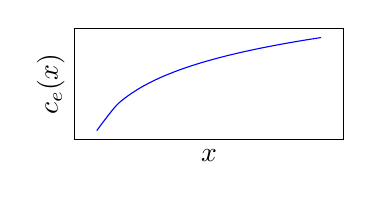
\begin{tikzpicture}
          \begin{axis}[
              xlabel=$x$,
              ylabel=$c_{e}(x)$,
              smooth,
              width=5cm,
              height=3cm,
              ticks=none,
              no markers
            ]
              \addplot{ln(x)};
          \end{axis}
        \end{tikzpicture}
      \end{center}
    \item restrict players demands to a specific mathematical structure:
      Matroids
  \end{itemize}
\end{frame}

\begin{frame}
  \frametitle{Definition: Matroid}
  \begin{columns}
    \column{0.5\textwidth}
    \begin{equation*}
      M = (E, B)
    \end{equation*}
    \vspace{-0.8cm}
    \begin{itemize}
      \item $E$: ground-set
      \item $B$: set of bases
      \item \emph{basis exchange property}:
        \vspace{-1cm}
        \begin{center}
          \begin{align*}
            \forall &X, Y\in B:\\
            &\forall x\in (X\setminus Y)\\
            &\exists y\in (Y\setminus X):\\
            &\;(X\setminus \set{x})\cup\{y\}\in B
          \end{align*}
        \end{center}
    \end{itemize}
    \column{0.5\textwidth}
    \uncover<2->{Spanning trees:}
    \begin{center}
      \uncover<2->{\resizebox{0.8\textwidth}{!}{\begin{tikzpicture}
  \node[node] (A) {};
  \node[below=0.5 of A] (d1) {};
  \node[node, below=0.5 of d1] (B) {};
  \node[right=1 of A] (d2) {};
  \node[node, right=1 of d2] (D) {};
  \node[node] (C) at (d1-|d2) {};
  \node[node] (E) at (B-|D) {};

  \draw[edge, p1] (A) to (B);
  \draw[edge, p1] (A) to (C);
  \draw[edge, p1] (B) to (C);
  \draw[edge, p1] (C) to (D);
  \draw[edge, p1] (C) to (E);
\end{tikzpicture}
}\\[0.5cm]}
      \uncover<3->{\resizebox{0.4\textwidth}{!}{\begin{tikzpicture}
  \node[node] (A) {};
  \node[below=0.5 of A] (d1) {};
  \node[node, below=0.5 of d1] (B) {};
  \node[right=1 of A] (d2) {};
  \node[node, right=1 of d2] (D) {};
  \node[node] (C) at (d1-|d2) {};
  \node[node] (E) at (B-|D) {};

  \draw[edge, dotted, p1] (A) to (B);
  \draw[edge, p1] (A) to (C);
  \draw[edge, p1] (B) to (C);
  \draw[edge, p1] (C) to (D);
  \draw[edge, p1] (C) to (E);
\end{tikzpicture}
}}
      \uncover<4->{\resizebox{0.4\textwidth}{!}{\begin{tikzpicture}
  \node[node] (A) {};
  \node[below=0.5 of A] (d1) {};
  \node[node, below=0.5 of d1] (B) {};
  \node[right=1 of A] (d2) {};
  \node[node, right=1 of d2] (D) {};
  \node[node] (C) at (d1-|d2) {};
  \node[node] (E) at (B-|D) {};

  \draw[edge, p1] (A) to (B);
  \draw[edge, p1, dotted] (A) to (C);
  \draw[edge, p1] (B) to (C);
  \draw[edge, p1] (C) to (D);
  \draw[edge, p1] (C) to (E);
\end{tikzpicture}
}}
      \uncover<5->{\resizebox{0.4\textwidth}{!}{\begin{tikzpicture}
  \node[node] (A) {};
  \node[below=0.5 of A] (d1) {};
  \node[node, below=0.5 of d1] (B) {};
  \node[right=1 of A] (d2) {};
  \node[node, right=1 of d2] (D) {};
  \node[node] (C) at (d1-|d2) {};
  \node[node] (E) at (B-|D) {};

  \draw[edge, p1] (A) to (B);
  \draw[edge, p1] (A) to (C);
  \draw[edge, p1, dotted] (B) to (C);
  \draw[edge, p1] (C) to (D);
  \draw[edge, p1] (C) to (E);
\end{tikzpicture}
}}
    \end{center}
  \end{columns}
\end{frame}

\begin{frame}[fragile]
  \frametitle{Operations on Matroids $\mathcal{M} = \tupel{E, \mathcal{B}}$}
  \begin{columns}
    \column{0.5\textwidth}
    \begin{center}
      Contraction:
    \end{center}
    \vspace{-0.6cm}
    \begin{align*}
      &\mathcal{M}/e = \tupel{E\setminus\set{e}, \mathcal{B}/e}\text{ with}\\
      &\mathcal{B}/e = \set{B\subseteq (E\setminus\set{e})\middle| B\cup\set{e}\in\mathcal{B}}
    \end{align*}
    \column<4->{0.5\textwidth}
    \begin{center}
      Deletion:
    \end{center}
    \vspace{-0.6cm}
    \begin{align*}
      &\mathcal{M}\setminus e = \tupel{E\setminus\set{e},\mathcal{B}\setminus e}\text{ with}\\
      &\mathcal{B}\setminus e = \set{B\subseteq E\setminus\set{e}\middle|B\in\mathcal{B}}
    \end{align*}
  \end{columns}
  \begin{center}
    \begin{tikzpicture}
      \uncover<2->{\node (G) {\begin{tikzpicture}
  \node[node] (A) {};
  \node[below=0.5 of A] (d1) {};
  \node[node, below=0.5 of d1] (B) {};
  \node[right=1 of A] (d2) {};
  \node[node, right=1 of d2] (D) {};
  \node[node] (C) at (d1-|d2) {};
  \node[node] (E) at (B-|D) {};

  \draw[edge, p1] (A) to (B);
  \draw[edge, p1] (A) to (C);
  \draw[edge, p1] (B) to (C);
  \draw[edge, p1] (C) to (D);
  \draw[edge, p1] (C) to (E);
\end{tikzpicture}
};
      \node[right=1 of G] (leadsto) {\Huge$\leadsto$};}
      \uncover<3>{\node[right=1 of leadsto] (G') {\begin{tikzpicture}
  \node[node] (A) {};
  \node[below=0.5 of A] (d1) {};
  \node[node, below=0.5 of d1] (B) {};
  \node[right=1 of A] (d2) {};
  \node[node, right=1 of d2] (D) {};
  \node[node] (C) at (d1-|d2) {};
  \node[node] (E) at (B-|D) {};
  
  \node[fit=(A) (B), draw, rectangle, rounded corners, black] (new) {};

  \draw[edge, p1] (new) to (C);
  \draw[edge, p1, dotted] (A) to (C);
  \draw[edge, p1, dotted] (B) to (C);
  \draw[edge, p1] (A) to (B);
  \draw[edge, p1] (C) to (D);
  \draw[edge, p1] (C) to (E);
\end{tikzpicture}
};}
      \uncover<5>{\node[right=1 of leadsto] (G'') {\begin{tikzpicture}
  \node[node] (A) {};
  \node[below=0.5 of A] (d1) {};
  \node[node, below=0.5 of d1] (B) {};
  \node[right=1 of A] (d2) {};
  \node[node, right=1 of d2] (D) {};
  \node[node] (C) at (d1-|d2) {};
  \node[node] (E) at (B-|D) {};

  \node[above left =0.1 and 0.1 of d1] (del1) {};
  \node[above right=0.1 and 0.1 of d1] (del2) {};
  \node[below left =0.1 and 0.1 of d1] (del3) {};
  \node[below right=0.1 and 0.1 of d1] (del4) {};

  \draw[edge, p1, dotted] (A) to (B);
  \draw[edge, p1] (A) to (C);
  \draw[edge, p1] (B) to (C);
  \draw[edge, p1] (C) to (D);
  \draw[edge, p1] (C) to (E);

  \draw[thick, black] (del1) to (del4);
  \draw[thick, black] (del2) to (del3);
\end{tikzpicture}
};}
    \end{tikzpicture}
  \end{center}
\end{frame}

\subsection{Pure Nash equilibria}
\begin{frame}
  % \begin{itemize}
  %   \item (1 slide)
  %   \item Explain what PNEs are (maybe from previous presentations this
  %     knowledge can be assumed)
  %   \item Again the example can be used to illustrate what uniliteral change
  %     might imply
  % \end{itemize}
% \end{frame}
% \subsection{Basic matroid theory}
% \begin{frame}
  % \begin{itemize}
  %   \item (2/3 slides)
  %   \item Formally define matroids
  %   \item Explain the meaning of the definition by using the example
  %   \item Contraction and deletion (again with example)
  %   \item Define Matroid games (and mention that the example fits)
  % \end{itemize}
\end{frame}

\section{Algorithm: PNE in Unweighted Matroid Games}
\subsection{Algorithm}
\begin{frame}
  % \begin{itemize}
  %   \item Present algorithm (2 slides)
  %   \item Execute one or two steps at example (only a slide but animation might
  %     take some time ca. 5 minutes)
  % \end{itemize}
\end{frame}

\subsection{Correctness}
\begin{frame}
  % \begin{itemize}
  %   \item Intuitively present the ideas for the correctness (1/2 slides)
  %   \item (Formal proofs might take too long?)
  % \end{itemize}
\end{frame}

\section{Weighted Matroid Games}
\begin{frame}
  % \begin{itemize}
  %   \item (2 slides)
  %   \item Introduce socially optimal solution
  %   \item Show (or at least motivate) why this is a PNE
  %   \item Mention reduction to show that finding an optimal solution is NP-hard
  % \end{itemize}
\end{frame}

\section{Non-Matroid Strategy Spaces}
\subsection{Lack of PNE}
\begin{frame}
  % \begin{itemize}
  %   \item (1 slide)
  %   \item Present that for Non-Matroid Games we can find strategy spaces
  %     which do not allow PNE
  %   \item Illustrate the construction by a picture
  % \end{itemize}
\end{frame}

\subsection{Non-Decreasing Marginal Cost Functions \& Price of Anarchy}
\begin{frame}
  % \begin{itemize}
  %   \item (3 slides)
  %   \item Present that games with Non-Decreasing Marginal Cost Functions allow
  %     PNE (explain how the marginal cost pricing is obtained)
  %   \item Define Price of Anarchy
  %   \item Mention that non-increasing and non-decreasing games with weighted
  %     players is unbounded
  % \end{itemize}
\end{frame}

\section{Conclusion}
\begin{frame}
  % \begin{itemize}
  %   \item (1 slide)
  %   \item Sum up results
  %   \item Embed results into topic
  % \end{itemize}
\end{frame}

\end{document}
